%%%%%%%%%%%%%%%%%%%%%%%%%%%%%%%%%%%%%%%%%%%%%%%%%%%%%%%%%%%%%%%
%
% Welcome to Overleaf --- just edit your LaTeX on the left,
% and we'll compile it for you on the right. If you open the
% 'Share' menu, you can invite other users to edit at the same
% time. See www.overleaf.com/learn for more info. Enjoy!
%
%%%%%%%%%%%%%%%%%%%%%%%%%%%%%%%%%%%%%%%%%%%%%%%%%%%%%%%%%%%%%%%
% Block Diagram in LaTeX: Step-by-Step TikZ Tutorial
% Latexdraw.com
% 18/01/2020, 22:19

\documentclass[border=0.2cm]{standalone}

% More defined colors
\usepackage[dvipsnames]{xcolor}

% Required package
\usepackage{tikz}
\usetikzlibrary{positioning}


\begin{document}

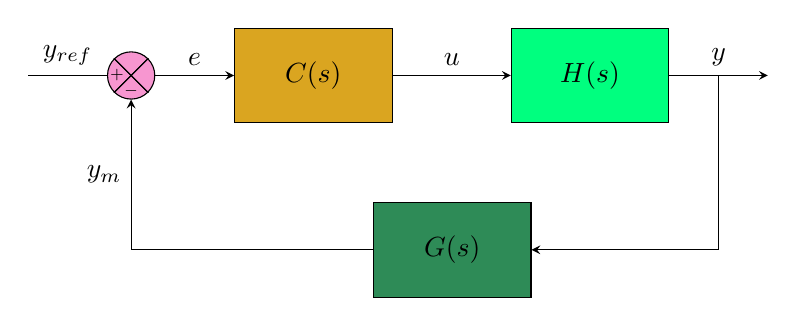
\begin{tikzpicture}

% Sum shape
\node[draw,
	circle,
	minimum size=0.6cm,
	fill=Rhodamine!50
] (sum) at (0,0){};

\draw (sum.north east) -- (sum.south west)
	(sum.north west) -- (sum.south east);

\draw (sum.north east) -- (sum.south west)
(sum.north west) -- (sum.south east);

\node[left=-1pt] at (sum.center){\tiny $+$};
\node[below] at (sum.center){\tiny $-$};

% Controller
\node [draw,
	fill=Goldenrod,
	minimum width=2cm,
	minimum height=1.2cm,
	right=1cm of sum
]  (controller) {$C(s)$};

% System H(s)
\node [draw,
	fill=SpringGreen, 
	minimum width=2cm, 
	minimum height=1.2cm,
	right=1.5cm of controller
] (system) {$H(s)$};

% Sensor block
\node [draw,
	fill=SeaGreen, 
	minimum width=2cm, 
	minimum height=1.2cm, 
	below right= 1cm and -0.25cm of controller
]  (sensor) {$G(s)$};

% Arrows with text label
\draw[-stealth] (sum.east) -- (controller.west)
	node[midway,above]{$e$};

\draw[-stealth] (controller.east) -- (system.west) 
	node[midway,above]{$u$};

\draw[-stealth] (system.east) -- ++ (1.25,0) 
	node[midway](output){}node[midway,above]{$y$};

\draw[-stealth] (output.center) |- (sensor.east);

\draw[-stealth] (sensor.west) -| (sum.south) 
	node[near end,left]{$y_m$};

\draw (sum.west) -- ++(-1,0) 
	node[midway,above]{$y_{ref}$};


\end{tikzpicture}




    %%Marco
    Montaggio del setup sperimentale e familiarizzazione col convertitore e con la
    strumentazione
    2. Analisi del funzionamento del modulatore PWM
    3. Verifica del funzionamento statico del convertitore
    • Analisi delle forme d’onda di tensione e corrente in DCM e CCM e identificazione
    del limite tra funzionamento CCM e DCM e confronto tra diodo
    veloce e diodo lento
    • Tracciamento delle caratteristiche di uscita (rapporto di conversione in
    funzione della corrente di carico a duty cycle costante)
\end{document}